\chapter{Results}
\label{chap:result}

\section{Data collection}
Tickers was 

News articles were scraped on a per stock ticker basis from Reuters. The implementation follows the stpes described in \ref{sec:news}. 

\section{Data Classification}
bla

\section{Event Study}
\subsection{All Events}
Overall, the event study shows that the impact of security incidents on stock prices is negative, with a statistical significance at the 0.05 level. The CAAR for all the 161 identified unique events was -1.6 per cent after ten days and -3.5 per cent after 50 days. This can be seen in table \ref{tab:esAll} and figure \ref{fig:esAll} for the 15 day event window, and table \ref{tab:esAllLong} and figure \ref{fig:esAllLong} for the 75 day event window. Interestingly, as can be seen from figure \ref{fig:esAll} the impact is notable sometime before the event date. There are two possible explanations for the earlier observed impact. One is that news agencies are not the first to discover the information regarding security incidents. The second is that one security incident might have multiple news articles written about it, thus shifting the aggregate observed impact on the event window timeline. Both explanations are likely to be present. The event study also shows what we would expect regarding removing random noise. When looking at the 75-day event window in figure \ref{fig:esAllLong} the CAAR line tracks the market until it gets close to the event date, and then it starts to drop until it again stabilises and starts tracking the market again.


\begin{figure}[h]
  \centering
  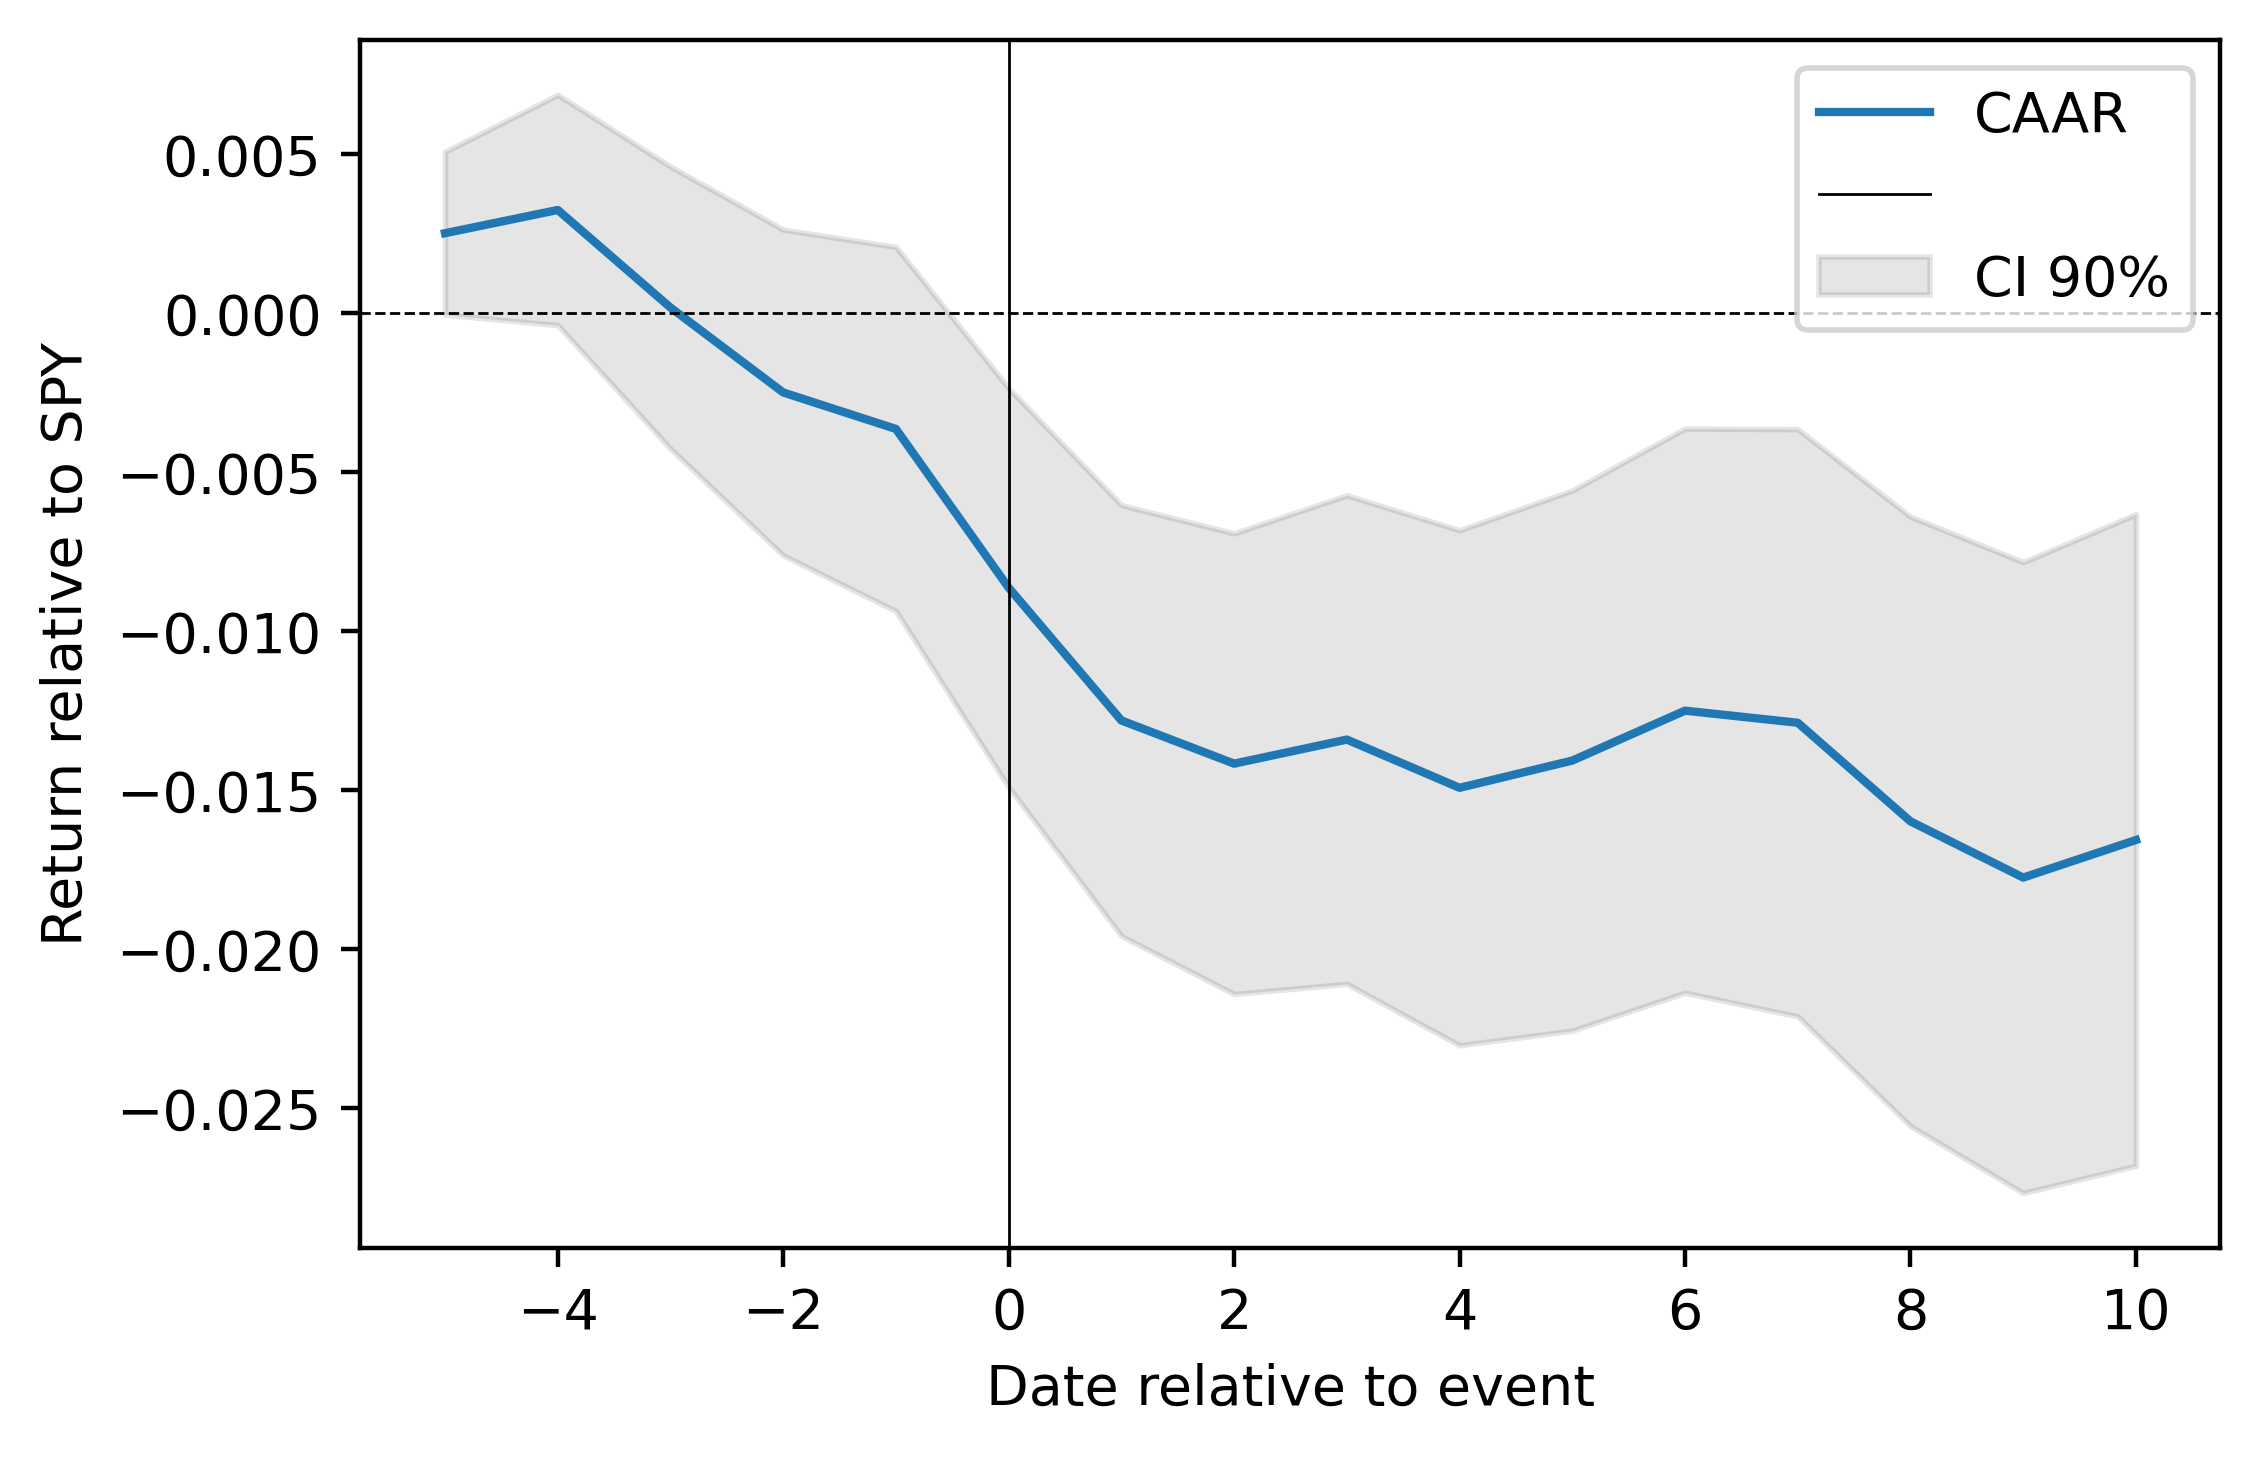
\includegraphics[width=1\textwidth]{figures/esAll.png}
  \caption{CAAR of all events. Event window: (-5, 10)}
  \label{fig:esAll}
\end{figure}



\begin{table}[h]
    \centering
    \caption{Event study of all events. Event window: (-5, 10)}
    \label{tab:esAll}
    \begin{tabular}{|c|c|c|c|c|c|c|}
        \hline
        \textbf{Day} & \textbf{AAR} & \textbf{Std. E. AAR} & \textbf{CAAR} & \textbf{Std. E. CAAR} & \textbf{T-stat} & \textbf{P-value} \\
        \hline
        \textbf{-5} & 0.003 & 0.002 & 0.003 & 0.00200 & 1.26 & 0.21 \\
        \hline
        \textbf{-4} & 0.001 & 0.002 & 0.003 & 0.00283 & 1.15 & 0.25 \\
        \hline
        \textbf{-3} & -0.003 & 0.002 & 0.0 & 0.00346 & 0.05 & 0.96 \\
        \hline
        \textbf{-2} & -0.003 & 0.002 & -0.002 & 0.00400 & -0.62 & 0.53 \\
        \hline
        \textbf{-1} & -0.001 & 0.002 & -0.004 & 0.00447 & -0.81 & 0.42 \\
        \hline
        \textbf{0} & -0.005 & 0.002 & -0.009 * & 0.00489 & -1.76 & 0.08 \\
        \hline
        \textbf{1} & -0.004 & 0.002 & -0.013 ** & 0.00529 & -2.42 & 0.02 \\
        \hline
        \textbf{2} & -0.001 & 0.002 & -0.014 ** & 0.00565 & -2.50 & 0.01 \\
        \hline
        \textbf{3} & 0.001 & 0.002 & -0.013 ** & 0.00599 & -2.24 & 0.03 \\
        \hline
        \textbf{4} & -0.002 & 0.002 & -0.015 ** & 0.00632 & -2.36 & 0.02 \\
        \hline
        \textbf{5} & 0.001 & 0.002 & -0.014 ** & 0.00663 & -2.12 & 0.03 \\
        \hline
        \textbf{6} & 0.002 & 0.002 & -0.012 * & 0.00692 & -1.80 & 0.07 \\
        \hline
        \textbf{7} & -0.000 & 0.002 & -0.013 * & 0.00720 & -1.79 & 0.07 \\
        \hline
        \textbf{8} & -0.003 & 0.002 & -0.016 ** & 0.00748 & -2.14 & 0.03 \\
        \hline
        \textbf{9} & -0.002 & 0.002 & -0.018 ** & 0.00774 & -2.29 & 0.02 \\
        \hline
        \textbf{10} & 0.001 & 0.002 & -0.017 ** & 0.00799 & -2.07 & 0.04 \\
        \hline

    \end{tabular}
\end{table}


\begin{figure}[h]
  \centering
  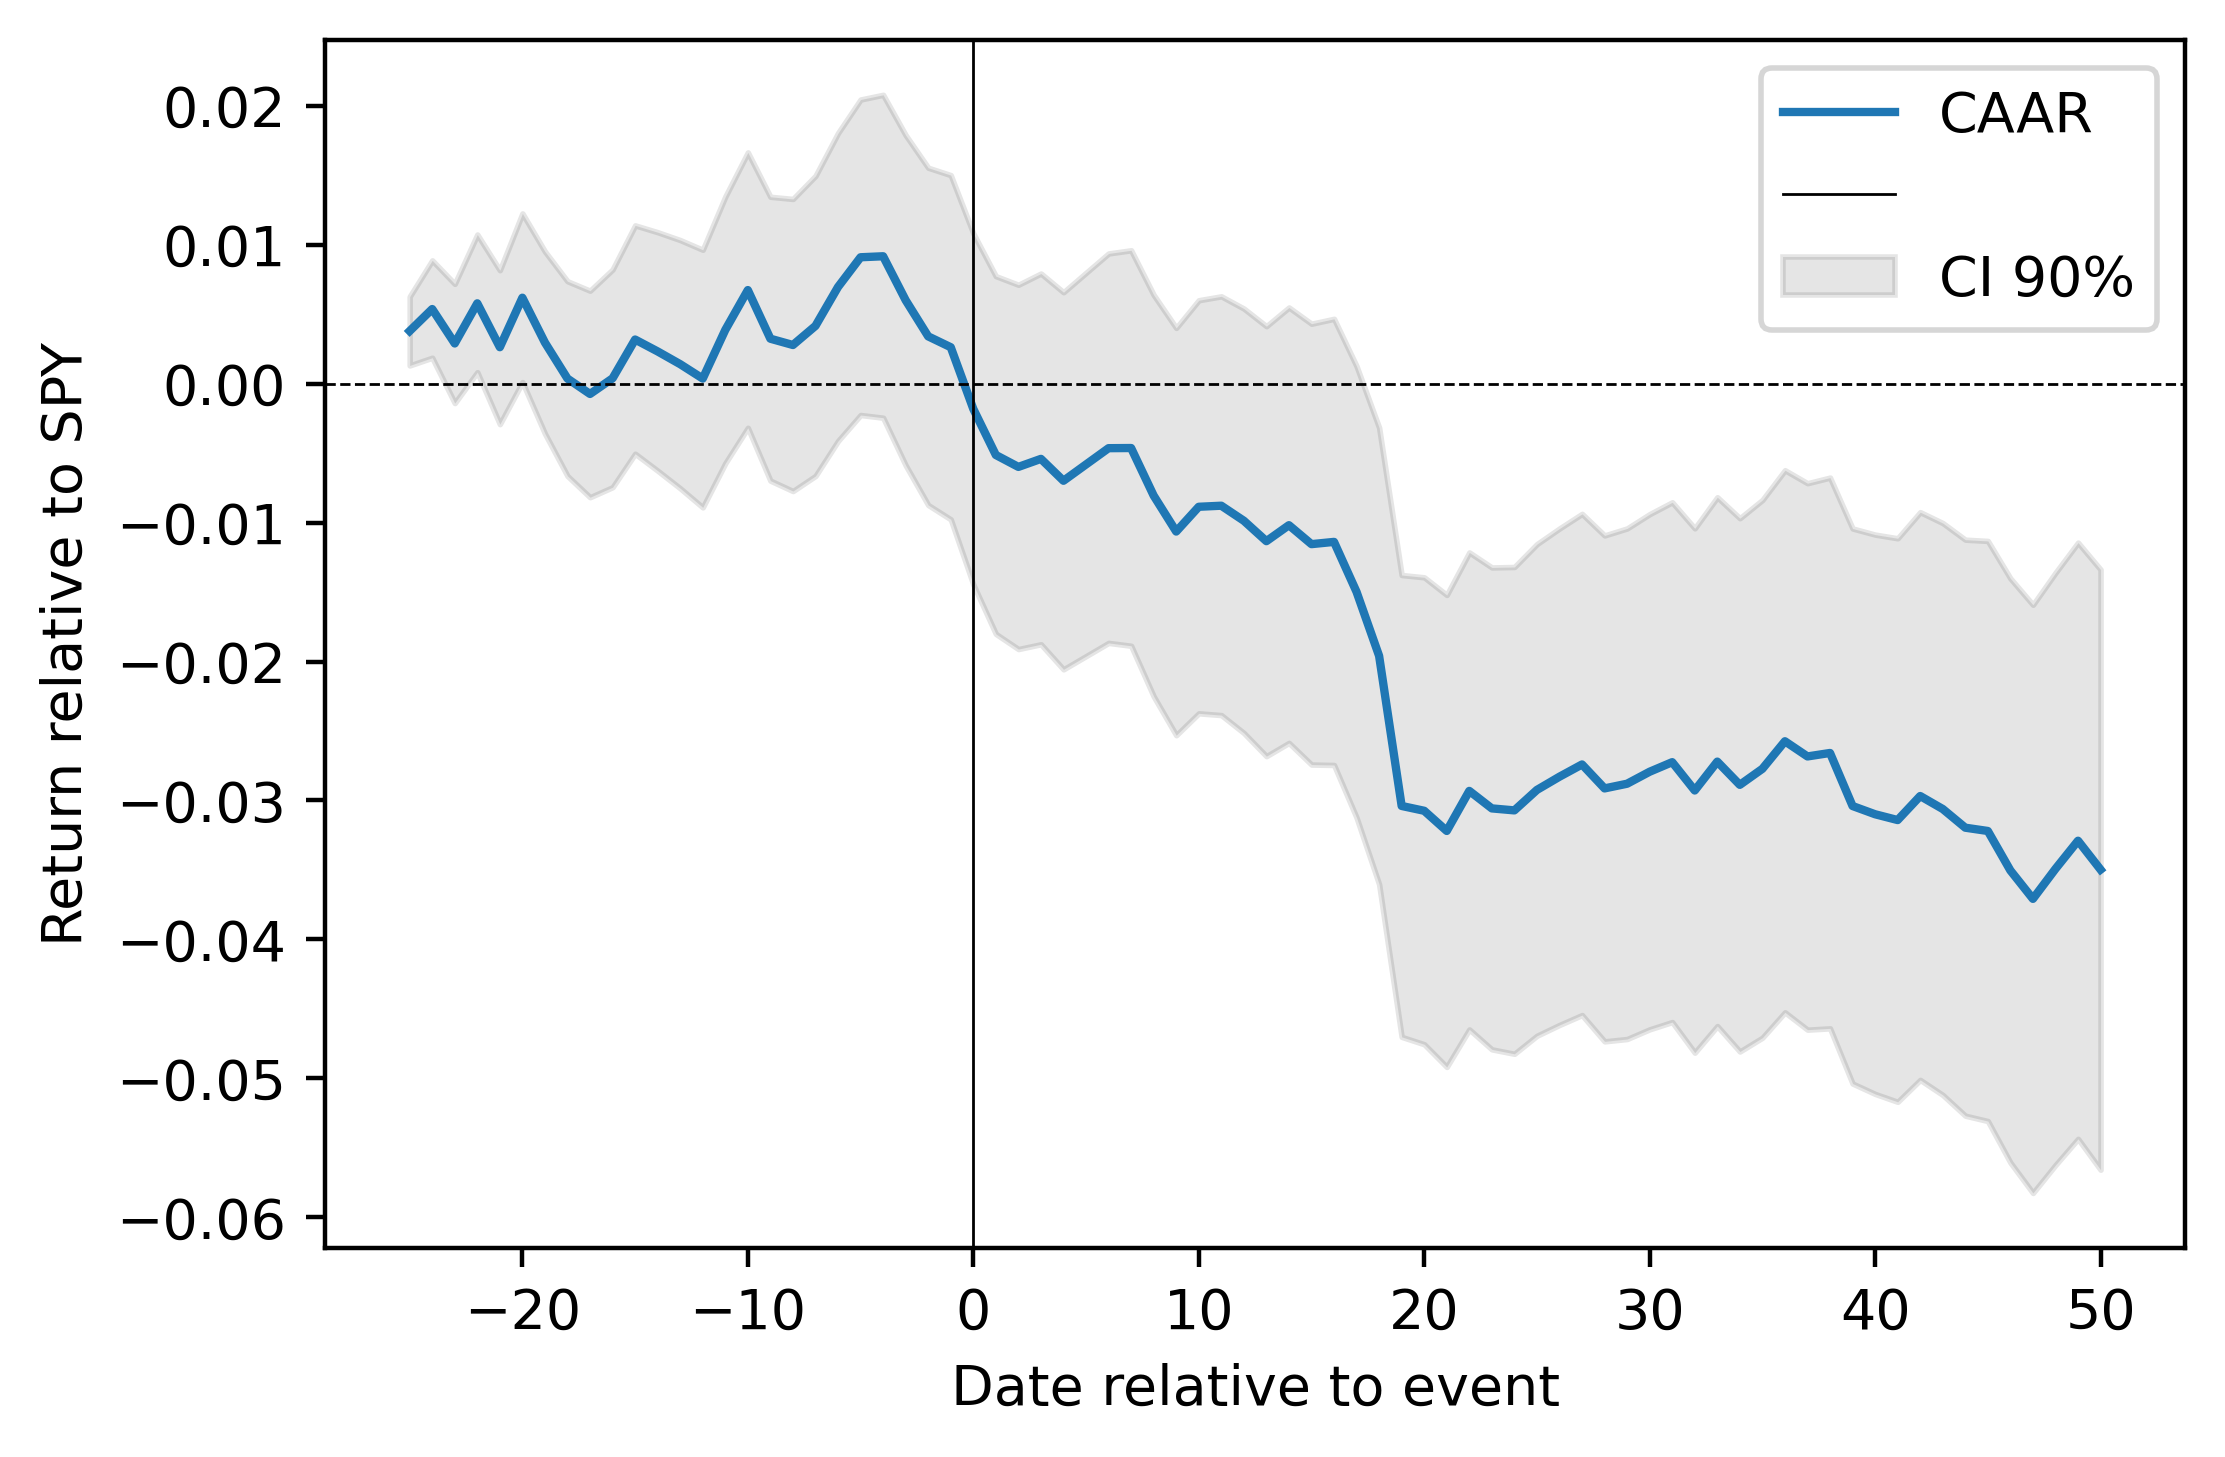
\includegraphics[width=1\textwidth]{figures/esAllLong.png}
  \caption{CAAR of all events. Event window: (-25, 50)}
  \label{fig:esAllLong}
\end{figure}

\begin{table}[h]
    \centering
    \caption{Event study of all events. Event window: (-25, 50)}
    \label{tab:esAllLong}
    \begin{tabular}{|c|c|c|c|c|c|c|}
        \hline
        \textbf{Day} & \textbf{AAR} & \textbf{Std. E. AAR} & \textbf{CAAR} & \textbf{Std. E. CAAR} & \textbf{T-stat} & \textbf{P-value} \\
        \hline
        \textbf{-25} & 0.004 & 0.00193 & 0.004 * & 0.00193 & 1.96 & 0.05 \\
        \hline
        \textbf{-24} & 0.002 & 0.00193 & 0.005 * & 0.00273 & 1.96 & 0.05 \\
        \hline
        \textbf{-23} & -0.002 & 0.00193 & 0.003 & 0.00335 & 0.86 & 0.39 \\
        \hline
        \textbf{-22} & 0.003 & 0.00193 & 0.006 & 0.00387 & 1.50 & 0.13 \\
        \hline
        \textbf{-21} & -0.003 & 0.00193 & 0.003 & 0.00432 & 0.61 & 0.54 \\
        \hline
        ... & ... & ... & ... & ... & ... & ... \\
        \hline
        \textbf{46} & -0.003 & 0.00193 & -0.035 ** & 0.01641 & -2.14 & 0.03 \\
        \hline
        \textbf{47} & -0.002 & 0.00193 & -0.037 ** & 0.01652 & -2.24 & 0.02 \\
        \hline
        \textbf{48} & 0.002 & 0.00193 & -0.035 ** & 0.01663 & -2.10 & 0.04 \\
        \hline
        \textbf{49} & 0.002 & 0.00193 & -0.033 * & 0.01674 & -1.96 & 0.05 \\
        \hline
        \textbf{50} & -0.002 & 0.00193 & -0.035 ** & 0.01686 & -2.08 & 0.04 \\
        \hline
    \end{tabular}
\end{table}

\subsection{Big Cap Tech Stocks}

A quarter of the input events are about large-cap tech firms. When reviewing the news articles that make up these events, they do not seem to represent a security incident in which the large-cap firms are heavily involved or affected. When isolating the events affecting these firms (Microsoft, Apple and Google), we get 42 events. When performing an event study on these events, we get table \ref{tab:esBigTech} and figure \ref{fig:esBigCap}, which shows that there is no statistically significant impact from the events on the stock price. This observation also holds true when looking at a longer event window as can be seen in figure \ref{fig:esBigCapLong} and table \ref{tab:esBigTechLong}.

Furthermore, when performing an event study with the events from large-cap tech stocks(Microsoft, Apple and Google) removed,see figure \ref{fig:esnoBigCap} and table \ref{tab:esNoBigTech}. This observation of no effect also holds true when moving to longer event windows as can be seen in figure \ref{fig:esnoBigCapLong} and table \ref{tab:esNoBigTechLong}. These results show that the impact of the events on the stock price is not significant for the larger firms that are heavily involved with technology. This fact also coincides with the observation that actual news events did not have the large tech firms as victims or heavily affected. This connection strengthens the hypothesis that we can retrieve security incidents from news articles and that the news articles are not just random noise. Still, at the same time, it highlights a case where the assumption that a large portion of events represents security incidents of material impact on the mentioned firm is not true.

\begin{figure}[h]
  \centering
  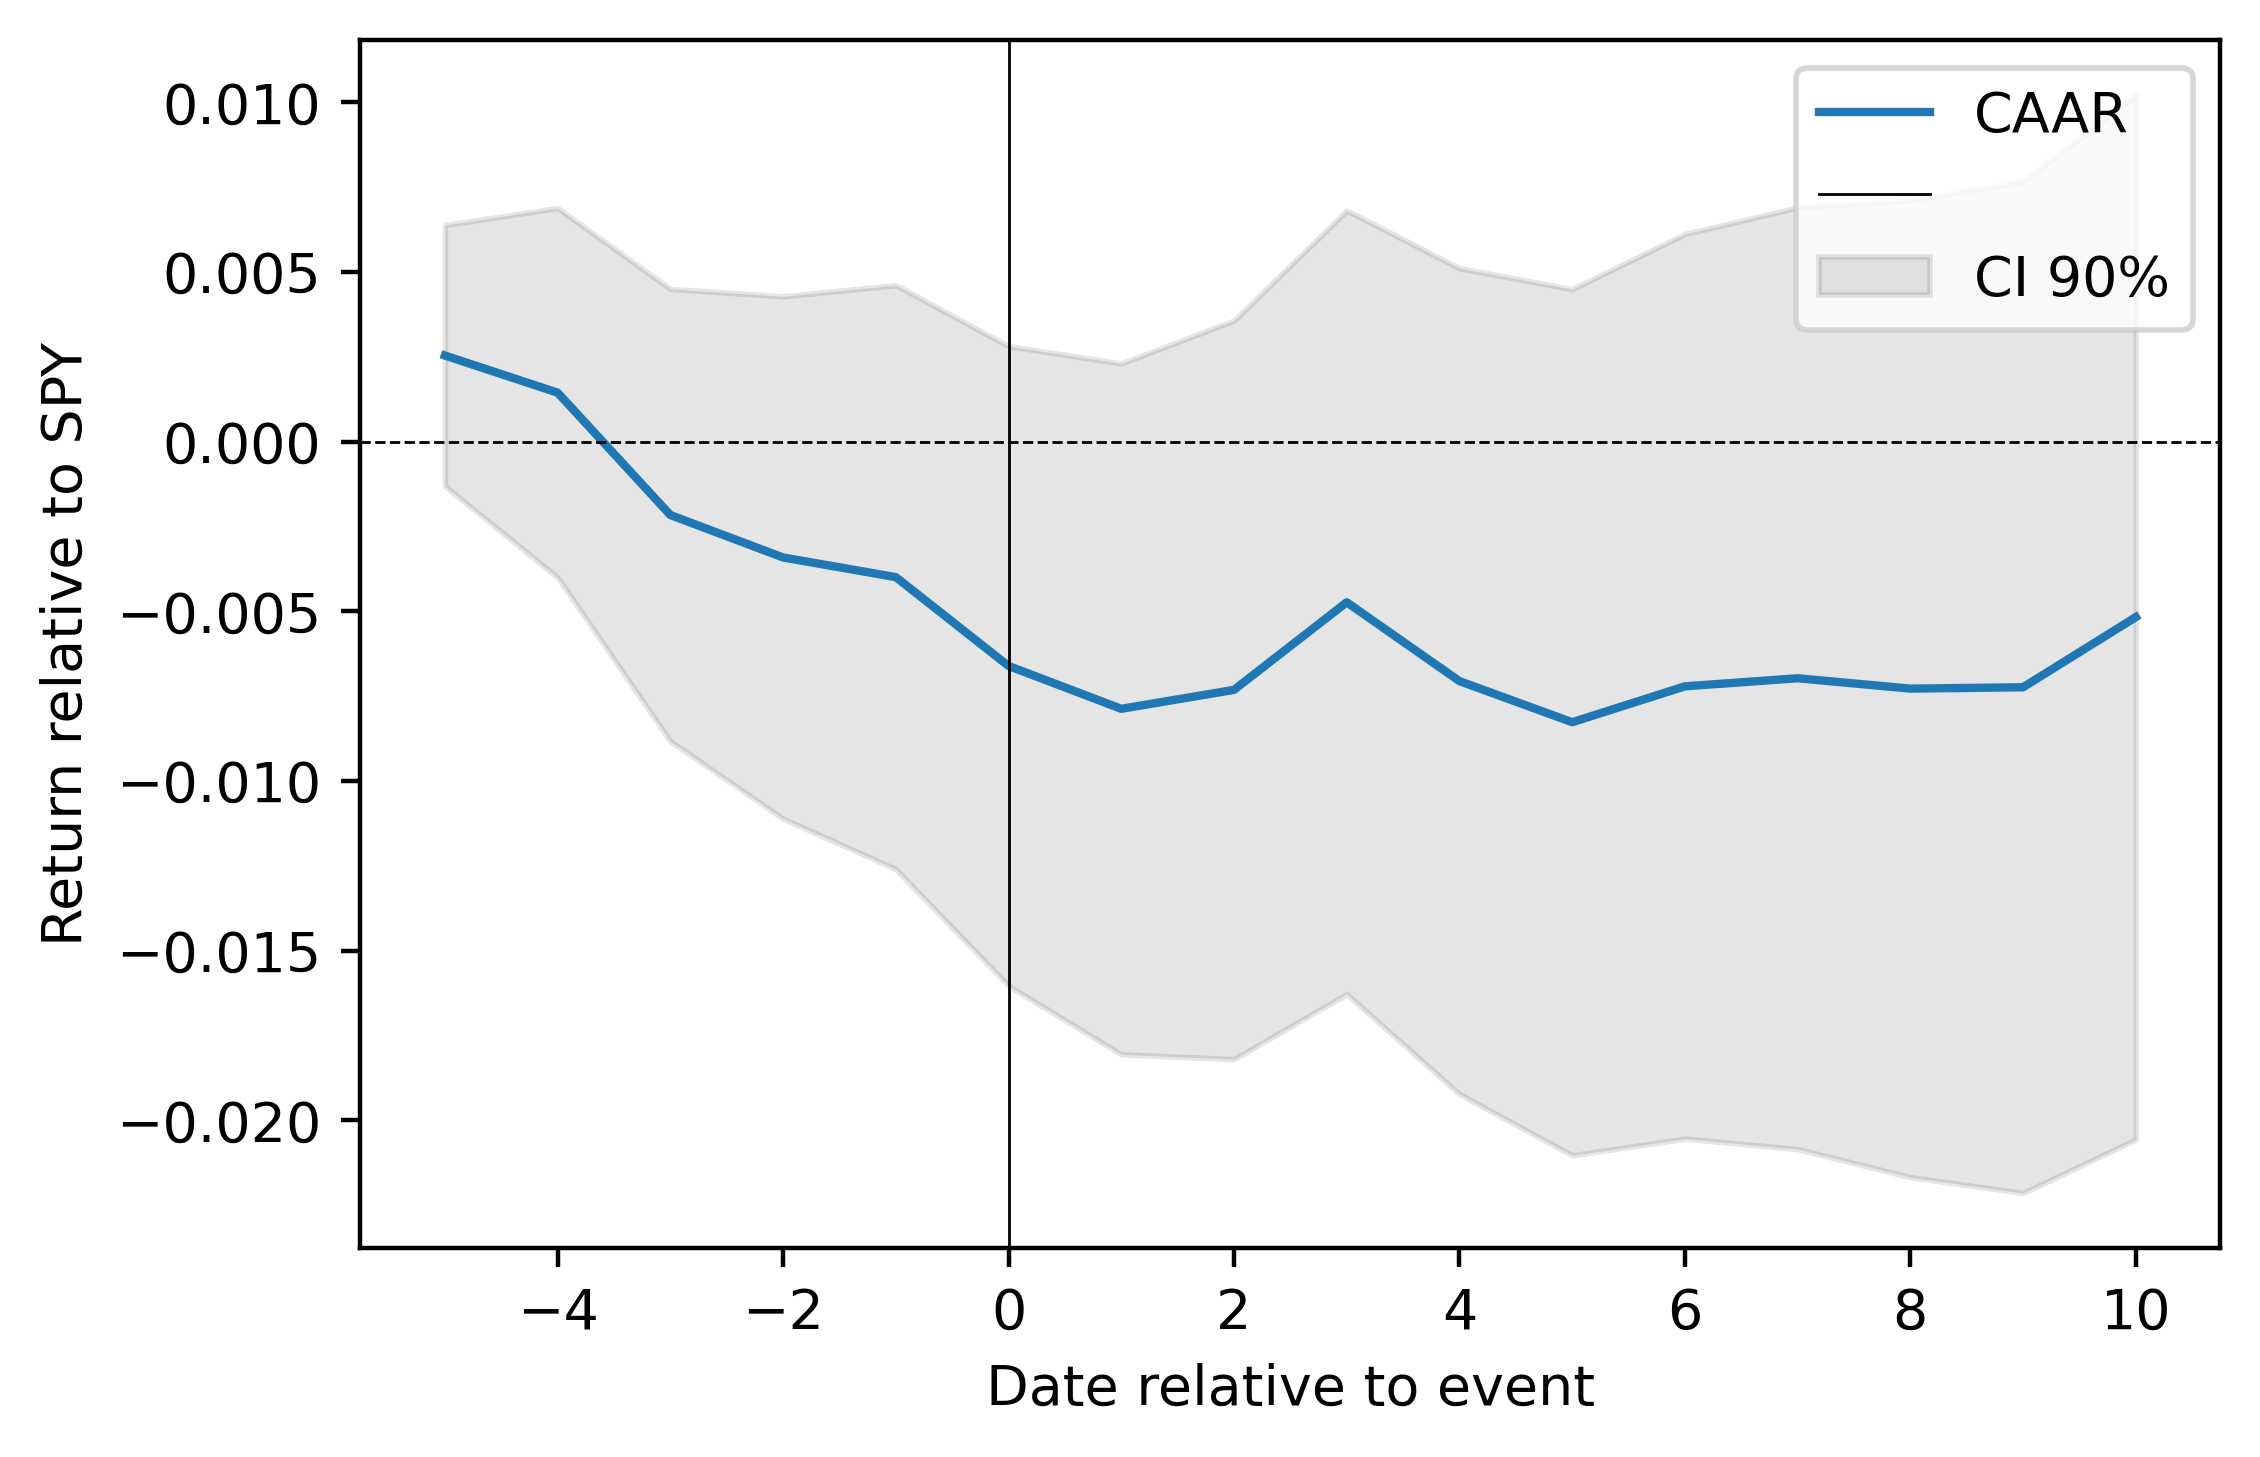
\includegraphics[width=1\textwidth]{figures/esBigCap.png}
  \caption{CAAR of big tech stock events. Event window: (-5, 10)}
  \label{fig:esBigCap}
\end{figure}


\begin{figure}[h]
  \centering
  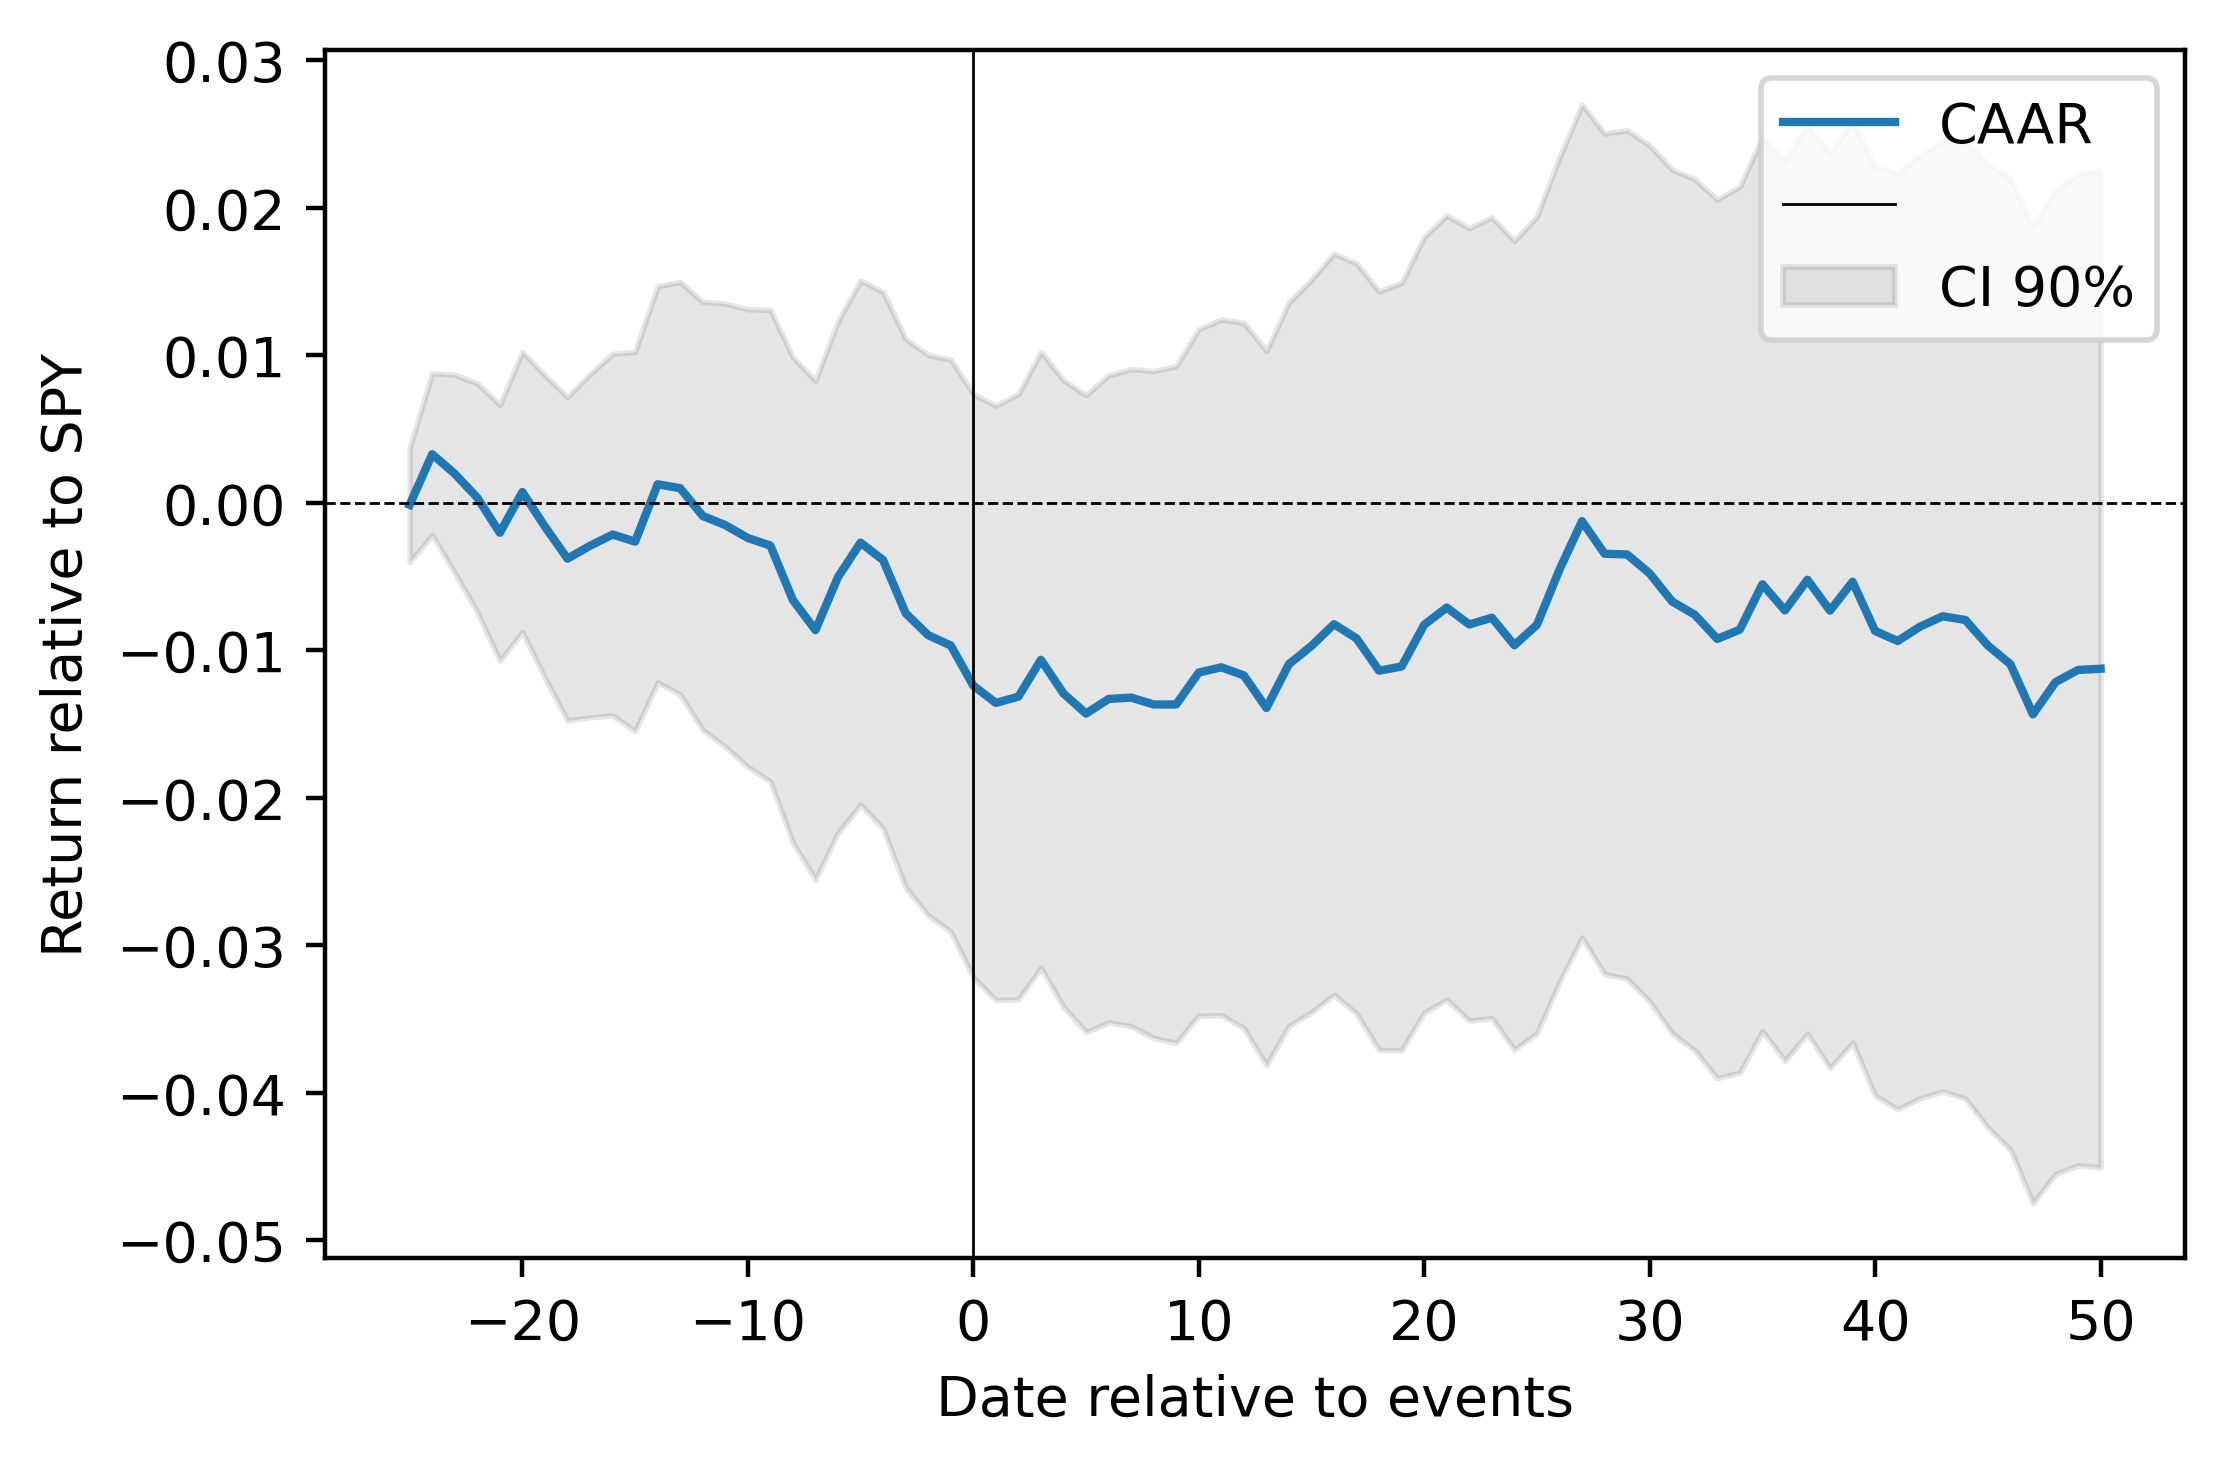
\includegraphics[width=1\textwidth]{figures/esBigCapLong.png}
  \caption{CAAR of big tech stock events. Event window: (-25, 50)}
  \label{fig:esBigCapLong}
\end{figure}

\begin{figure}[h]
  \centering
  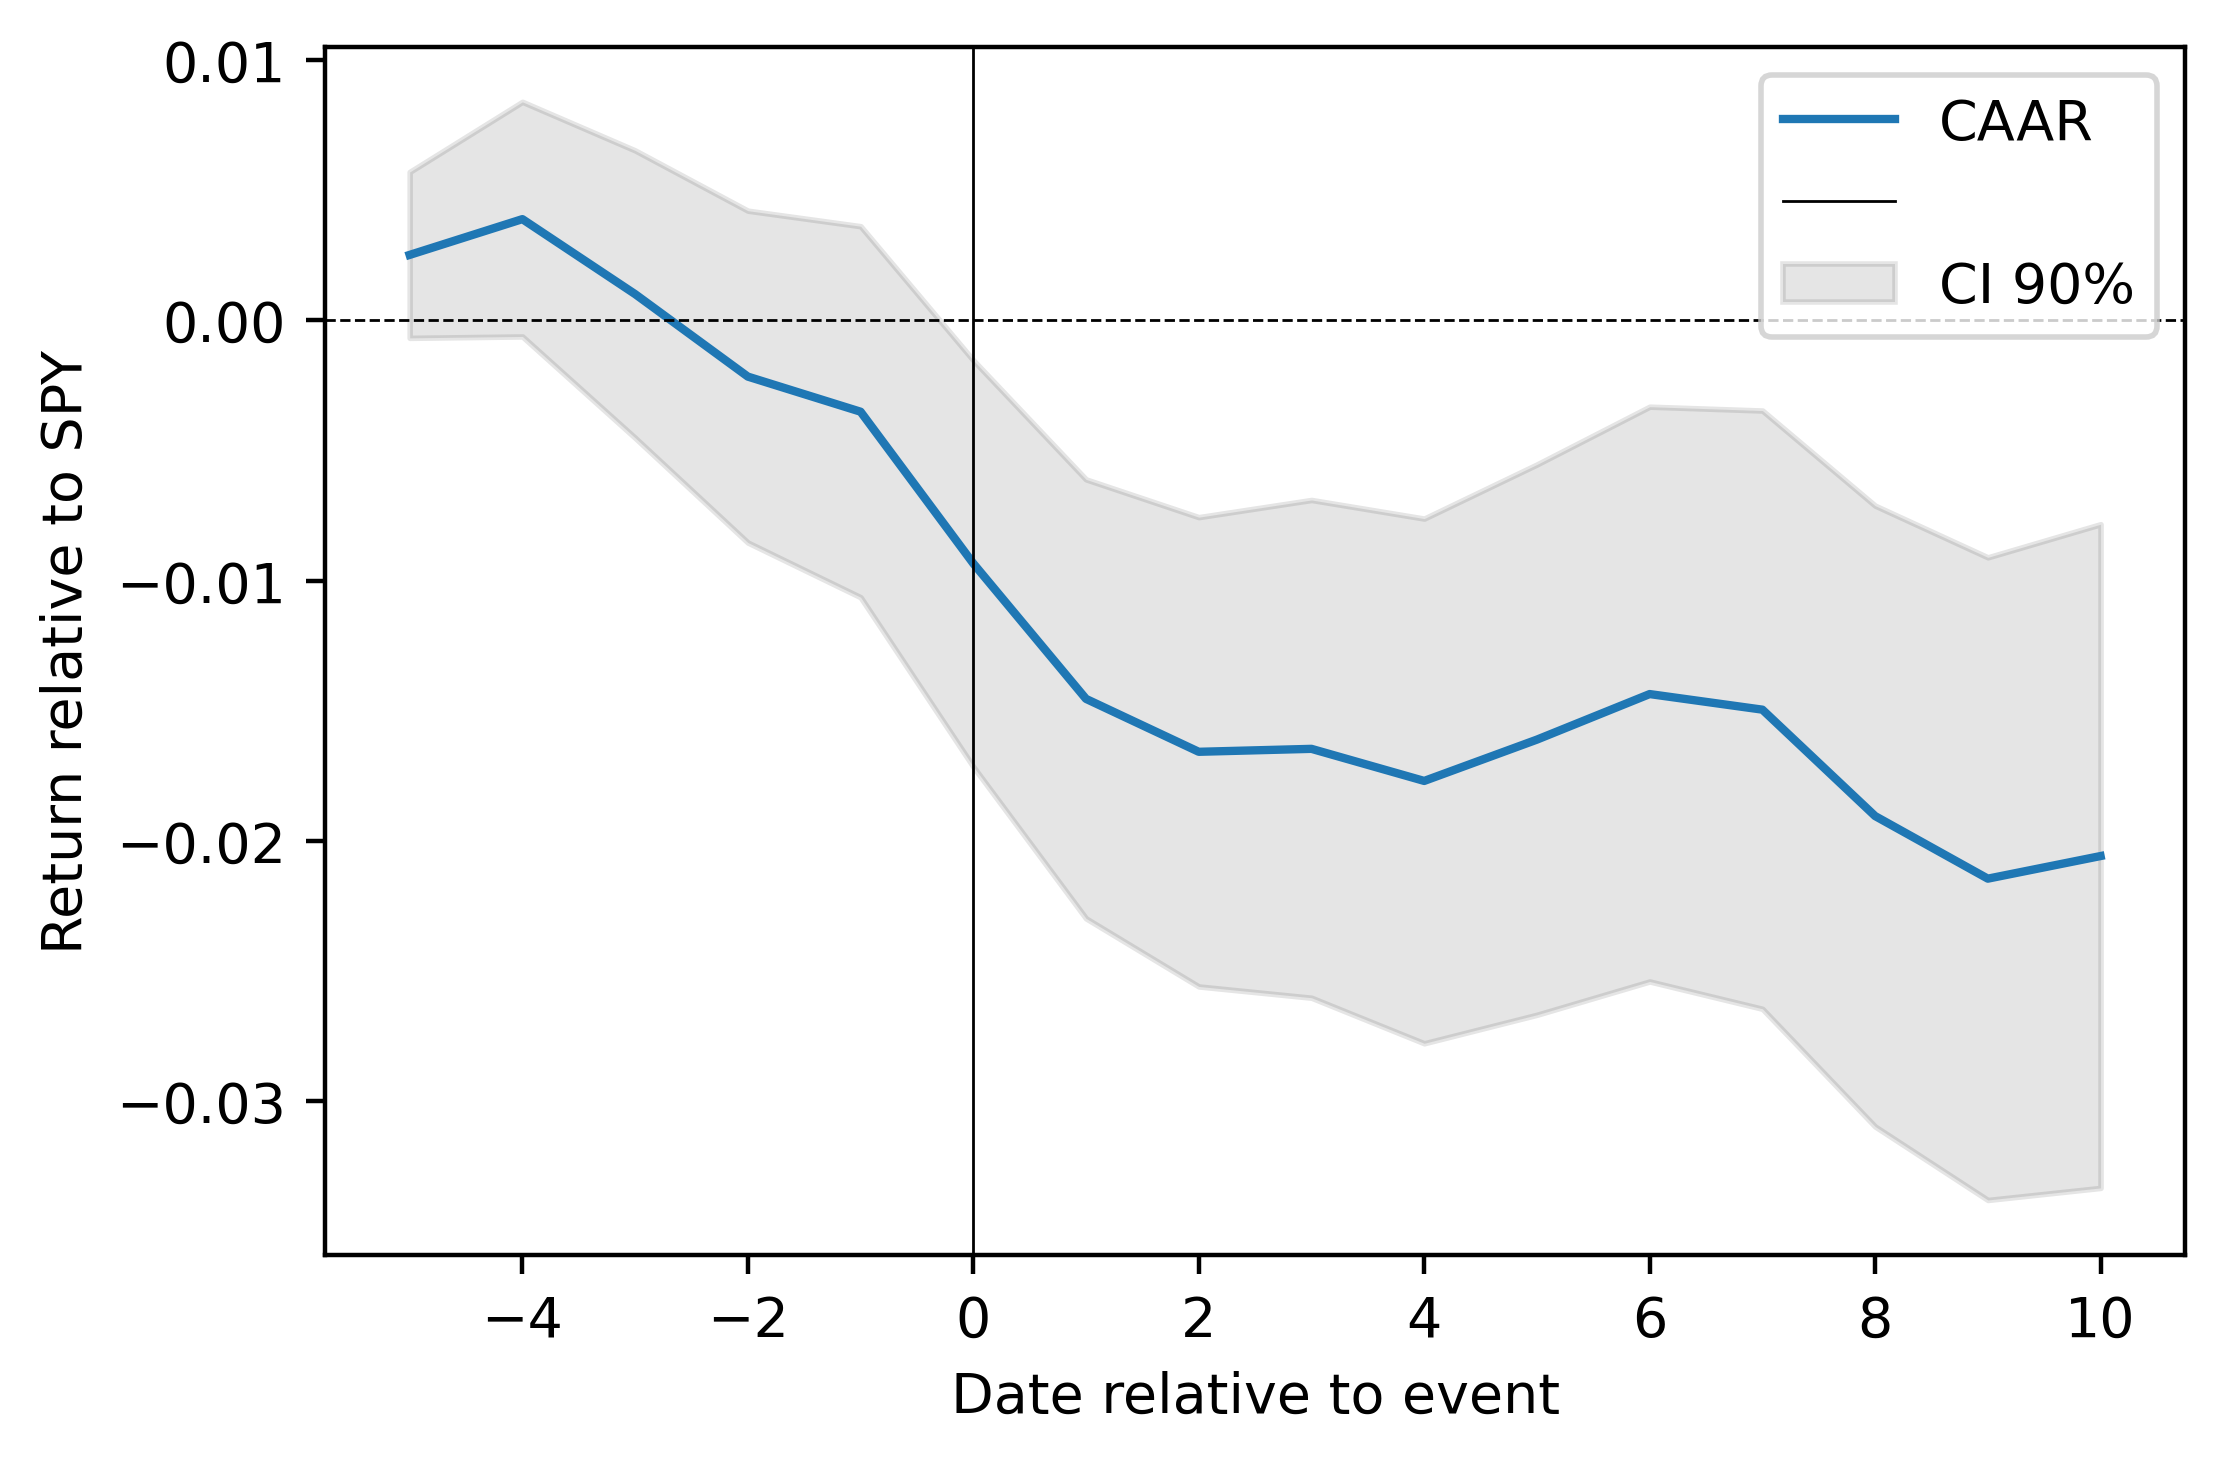
\includegraphics[width=1\textwidth]{figures/esnoBigCap.png}
  \caption{CAAR without big tech stock events. Event window: (-5, 10)}
  \label{fig:esnoBigCap}
\end{figure}


\begin{figure}[h]
  \centering
  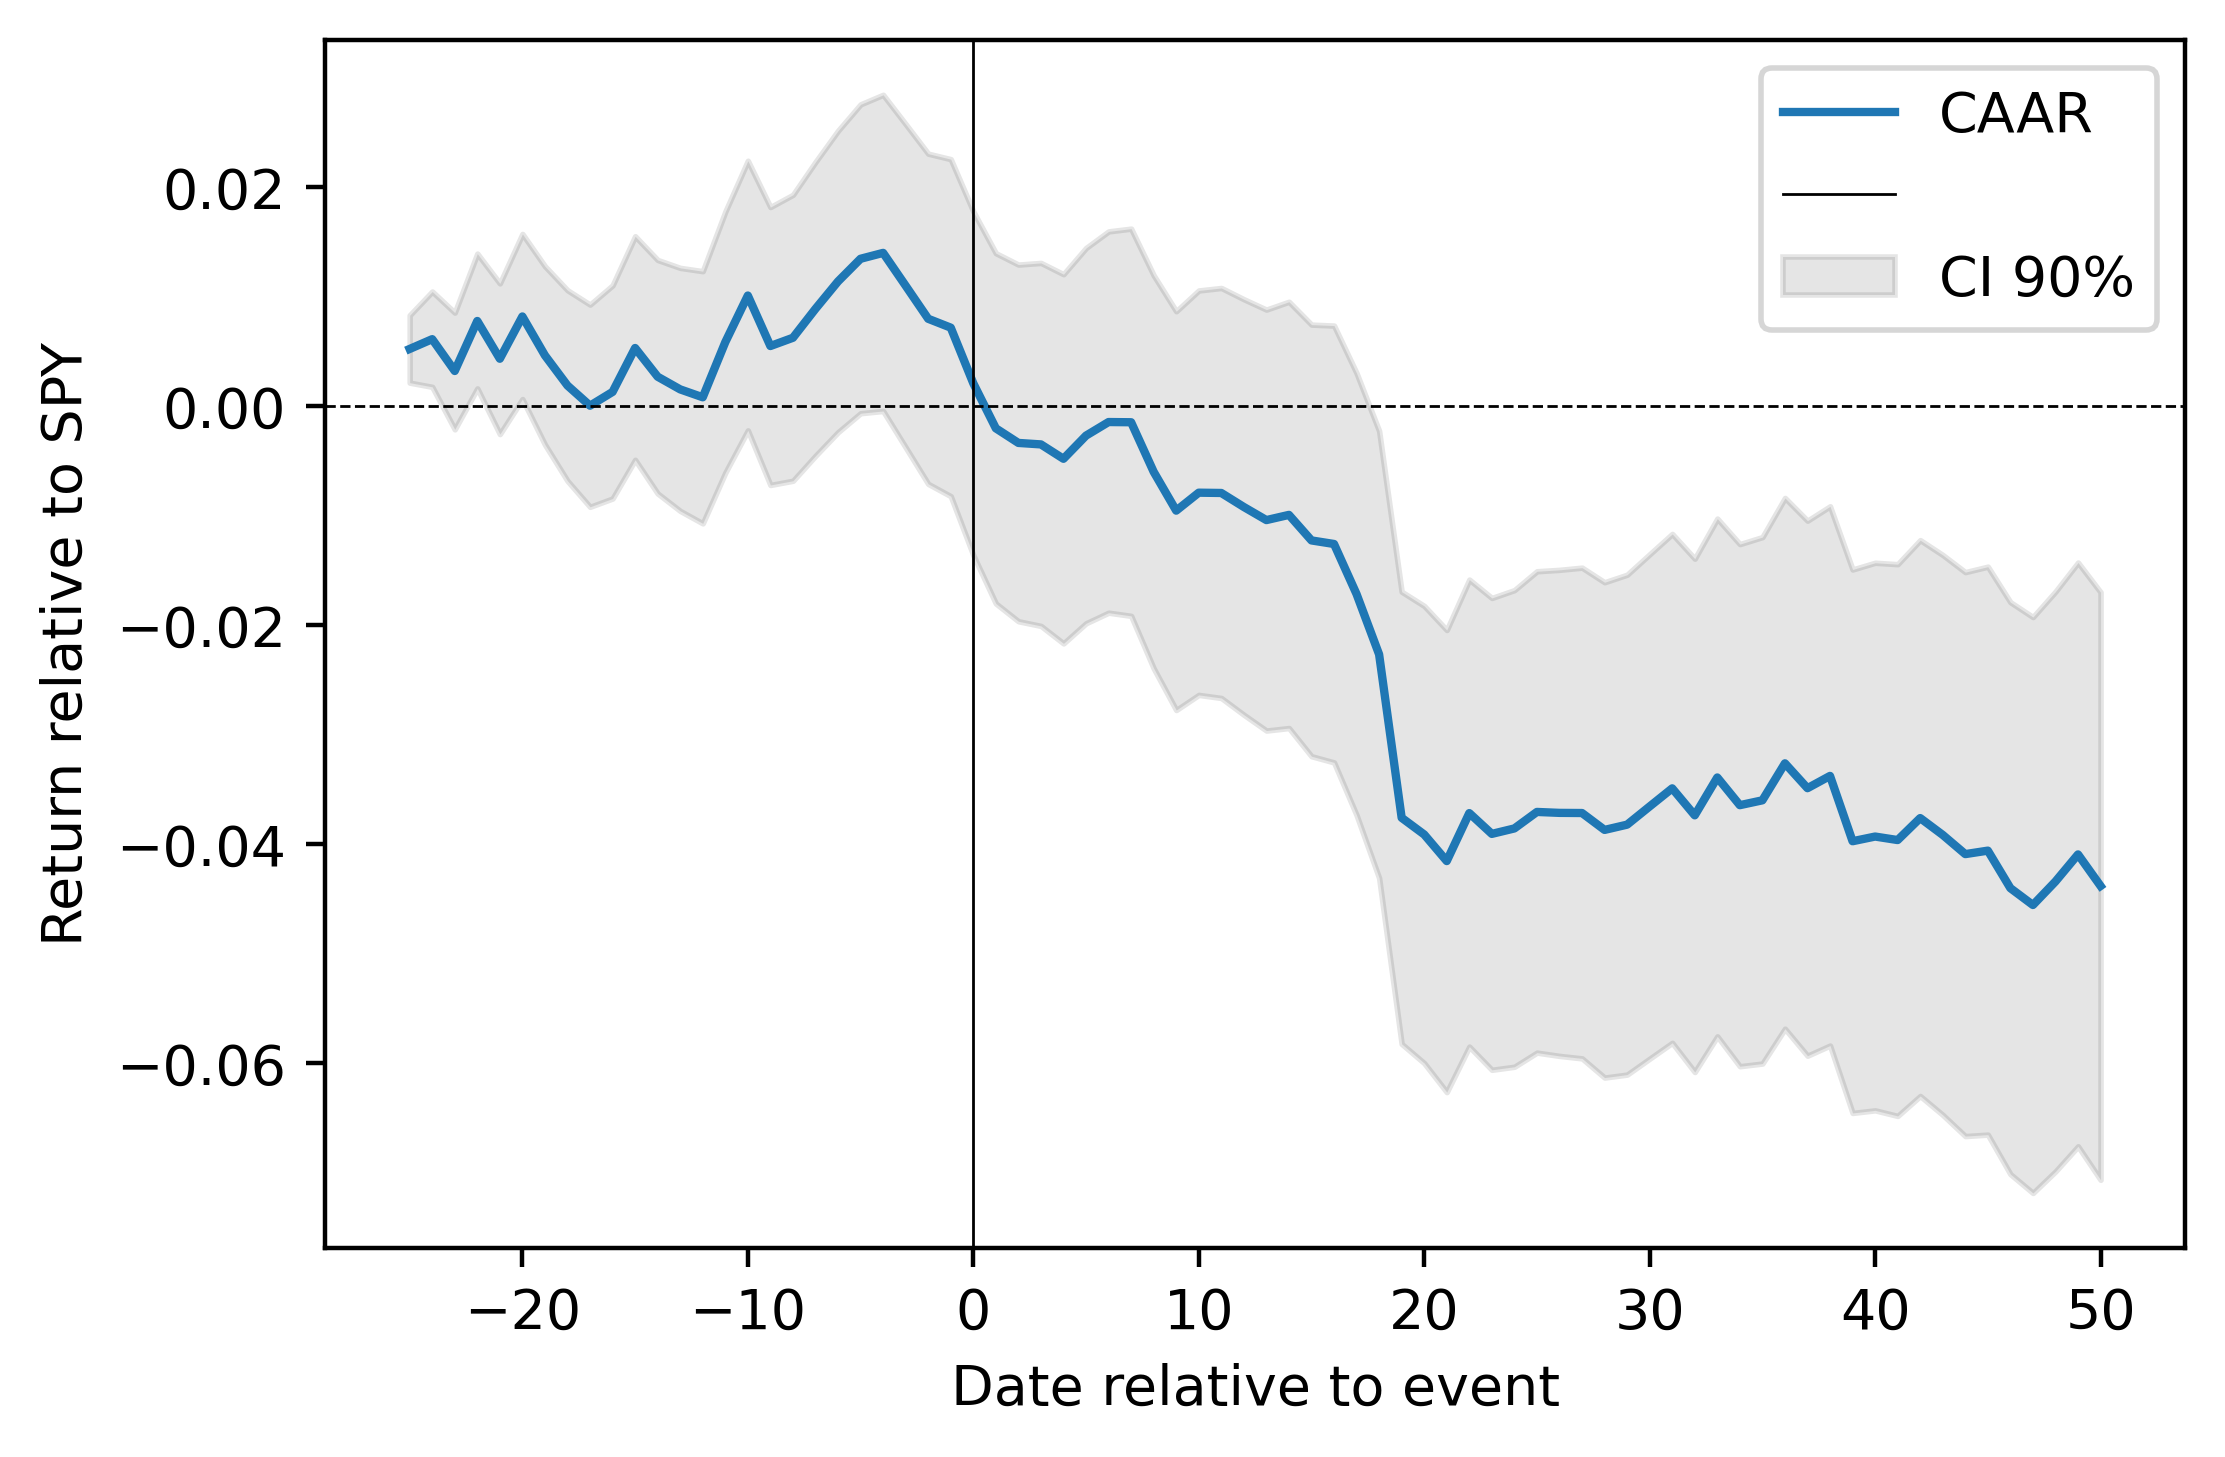
\includegraphics[width=1\textwidth]{figures/esnoBigCapLong.png}
  \caption{CAAR without big tech stock events. Event window: (-25, 50)}
  \label{fig:esnoBigCapLong}
\end{figure}




% returns
% Day AAR   Std. E. AAR CAAR    Std. E. CAAR    T-stat  P-value
% -5    0.003   0.00249 0.003   0.00249 1.01    0.31
% -4    0.001   0.00249 0.004   0.00352 1.11    0.27
% -3    -0.003  0.00249 0.001   0.00431 0.24    0.81
% -2    -0.003  0.00249 -0.002  0.00497 -0.43   0.66
% -1    -0.001  0.00249 -0.004  0.00556 -0.63   0.53
% 0 -0.006  0.00249 -0.009  0.00609 -1.53   0.13
% 1 -0.005  0.00249 -0.015 **   0.00658 -2.21   0.03
% 2 -0.002  0.00249 -0.017 **   0.00703 -2.36   0.02
% 3 0.000   0.00249 -0.016 **   0.00746 -2.21   0.03
% 4 -0.001  0.00249 -0.018 **   0.00787 -2.25   0.02
% 5 0.002   0.00249 -0.016 *    0.00825 -1.95   0.05
% 6 0.002   0.00249 -0.014  0.00862 -1.67   0.10
% 7 -0.001  0.00249 -0.015  0.00897 -1.67   0.10
% 8 -0.004  0.00249 -0.019 **   0.00931 -2.05   0.04
% 9 -0.002  0.00249 -0.021 **   0.00963 -2.23   0.03
% 10    0.001   0.00249 -0.021 **   0.00995 -2.07   0.04

\begin{table}[h]
    \centering
    \caption{Event study without big tech stock events. Event window: (-5, 10)}
    \label{tab:esNoBigTech}
    \begin{tabular}{|c|c|c|c|c|c|c|}
        \hline
        \textbf{Day} & \textbf{AAR} & \textbf{Std. E. AAR} & \textbf{CAAR} & \textbf{Std. E. CAAR} & \textbf{T-stat} & \textbf{P-value} \\
        \hline
        \textbf{-5} & 0.002 & 0.00193 & 0.003 & 0.00193 & 1.01 & 0.31 \\
        \hline
        \textbf{-4} & -0.001 & 0.002 & 0.004 & 0.003 & 1.11 & 0.27 \\
        \hline
        \textbf{-3} & -0.003 & 0.002 & 0.001 & 0.004 & 0.24 & 0.81 \\
        \hline
        \textbf{-2} & -0.003 & 0.002 & -0.002 & 0.005 & -0.43 & 0.66 \\
        \hline
        \textbf{-1} & -0.001 & 0.002 & -0.004 & 0.006 & -0.63 & 0.53 \\
        \hline
        \textbf{0} & -0.006 & 0.002 & -0.009 & 0.007 & -1.53 & 0.13 \\
        \hline
        \textbf{1} & -0.005 & 0.002 & -0.015 ** & 0.008 & -2.20 & 0.03 \\
        \hline
        \textbf{2} & -0.002 & 0.002 & -0.017 ** & 0.009 & -2.36 & 0.03 \\
        \hline
        \textbf{3} & 0.000 & 0.002 & -0.017 ** & 0.01 & -2.21 & 0.03 \\
        \hline
        \textbf{4} & -0.001 & 0.002 & -0.018 ** & 0.011 & -2.25 & 0.03 \\
        \hline
        \textbf{5} & 0.002 & 0.002 & -0.017 * & 0.012 & -1.95 & 0.05 \\
        \hline
        \textbf{6} & 0.002 & 0.002 & -0.015 & 0.013 & -1.67 & 0.10 \\
        \hline
        \textbf{7} & -0.001 & 0.002 & -0.015 & 0.014 & -1.67 & 0.10 \\
        \hline
        \textbf{8} & -0.004 & 0.002 & -0.019 ** & 0.015 & -2.05 & 0.04 \\
        \hline
        \textbf{9} & -0.002 & 0.002 & -0.021 ** & 0.016 & -2.23 & 0.03 \\
        \hline
        \textbf{10} & 0.001 & 0.002 & -0.021 ** & 0.017 & -2.07 & 0.04 \\
        \hline
    \end{tabular}
\end{table}

% returns
% Days  AAR Std. E. AAR CAAR    Std. E. CAAR    T-stat  P-value
% -25   0.005   0.0024  0.005 **    0.00240 2.19    0.03
% -24   0.001   0.0024  0.006 * 0.00340 1.81    0.07
% -23   -0.003  0.0024  0.003   0.00416 0.78    0.44
% -22   0.005   0.0024  0.008   0.00480 1.62    0.10
% -21   -0.003  0.0024  0.004   0.00537 0.81    0.42
% ...   ... ... ... ... ... ...
% 46    -0.003  0.0024  -0.044 **   0.02038 -2.16   0.03
% 47    -0.002  0.0024  -0.046 **   0.02052 -2.22   0.03
% 48    0.002   0.0024  -0.043 **   0.02066 -2.10   0.04
% 49    0.002   0.0024  -0.041 *    0.02080 -1.97   0.05
% 50    -0.003  0.0024  -0.044 **   0.02094 -2.09   0.04

\begin{table}[h]
    \centering
    \caption{Event study without big tech stock events. Event window: (-25, 50)}
    \label{tab:esNoBigTechLong}
    \begin{tabular}{|c|c|c|c|c|c|c|}
        \hline
        \textbf{Day} & \textbf{AAR} & \textbf{Std. E. AAR} & \textbf{CAAR} & \textbf{Std. E. CAAR} & \textbf{T-stat} & \textbf{P-value} \\
        \hline
        \textbf{-25} & 0.005 & 0.0024 & 0.005 ** & 0.00240 & 2.19 & 0.03 \\
        \hline
        \textbf{-24} & 0.001 & 0.0024 & 0.006 * & 0.00340 & 1.81 & 0.07 \\
        \hline
        \textbf{-23} & -0.003 & 0.0024 & 0.003 & 0.00416 & 0.78 & 0.44 \\
        \hline
        \textbf{-22} & 0.005 & 0.0024 & 0.008 & 0.00480 & 1.62 & 0.10 \\
        \hline
        \textbf{-21} & -0.003 & 0.0024 & 0.004 & 0.00537 & 0.81 & 0.42 \\
        \hline
        ... & ... & ... & ... & ... & ... & ... \\
        \hline
        \textbf{46} & -0.003 & 0.0024 & -0.044 ** & 0.02038 & -2.16 & 0.03 \\
        \hline
        \textbf{47} & -0.002 & 0.0024 & -0.046 ** & 0.02052 & -2.22 & 0.03 \\
        \hline
        \textbf{48} & 0.002 & 0.0024 & -0.043 ** & 0.02066 & -2.10 & 0.04 \\
        \hline
        \textbf{49} & 0.002 & 0.0024 & -0.041 * & 0.02080 & -1.97 & 0.05 \\
        \hline
        \textbf{50} & -0.003 & 0.0024 & -0.044 ** & 0.02094 & -2.09 & 0.04 \\
        \hline
    \end{tabular}
\end{table}




% esBigTech
% returns
% Days    AAR   Std. E. AAR CAAR    Std. E. CAAR    T-stat  P-value
% -5    0.003   0.003   0.003   0.00300 0.84    0.40
% -4    -0.001  0.003   0.001   0.00425 0.34    0.73
% -3    -0.004  0.003   -0.002  0.00520 -0.42   0.68
% -2    -0.001  0.003   -0.003  0.00600 -0.57   0.57
% -1    -0.001  0.003   -0.004  0.00671 -0.59   0.55
% 0 -0.003  0.003   -0.007  0.00735 -0.90   0.37
% 1 -0.001  0.003   -0.008  0.00794 -0.99   0.32
% 2 0.001   0.003   -0.007  0.00849 -0.86   0.39
% 3 0.003   0.003   -0.005  0.00901 -0.53   0.60
% 4 -0.002  0.003   -0.007  0.00949 -0.74   0.46
% 5 -0.001  0.003   -0.008  0.00996 -0.83   0.41
% 6 0.001   0.003   -0.007  0.01040 -0.69   0.49
% 7 0.000   0.003   -0.007  0.01082 -0.64   0.52
% 8 -0.000  0.003   -0.007  0.01123 -0.65   0.52
% 9 0.000   0.003   -0.007  0.01163 -0.62   0.53
% 10    0.002   0.003   -0.005  0.01201 -0.43   0.67

\begin{table}[h]
    \centering
    \caption{Event study with big tech stock events. Event window: (-5, 10)}
    \label{tab:esBigTech}
    \begin{tabular}{|c|c|c|c|c|c|c|c|}
        \hline
        \textbf{Day} & \textbf{AAR} & \textbf{Std. E. AAR} & \textbf{CAAR} & \textbf{Std. E. CAAR} & \textbf{T-stat} & \textbf{P-value} \\
        \hline
        \textbf{-5} & 0.003 & 0.003 & 0.003 & 0.00300 & 0.84 & 0.40 \\
        \hline
        \textbf{-4} & -0.001 & 0.003 & 0.001 & 0.00425 & 0.34 &  0.73 \\
        \hline
        \textbf{-3} & -0.004 & 0.003 & -0.002 & 0.00520 & -0.42 & 0.68 \\
        \hline
        \textbf{-2} & -0.001 & 0.003 & -0.003 & 0.00600 & -0.57 & 0.57 \\
        \hline
        \textbf{-1} & -0.001 & 0.003 & -0.004 &  0.00671 & -0.59 & 0.55 \\
        \hline
        \textbf{0} & -0.003 & 0.003 & -0.007 & 0.00735 & -0.90 & 0.37 \\
        \hline
        \textbf{1} & -0.001 & 0.003 & -0.008 & 0.00794 & -0.99 & 0.32 \\
        \hline
        \textbf{2} & 0.001 & 0.003 & -0.007 & 0.00849 & -0.86 &  0.39 \\
        \hline
        \textbf{3} & 0.003 & 0.003 & -0.005 & 0.00901 & -0.53 & 0.60 \\
        \hline
        \textbf{4} & -0.002 & 0.003 & -0.007 & 0.00949 & -0.74 & 0.46 \\
        \hline
        \textbf{5} & -0.001 &  0.003 & -0.008 & 0.00996 & -0.83 &  0.41 \\
        \hline
        \textbf{6} & 0.001 & 0.003 & -0.007 &  0.01040 & -0.69 & 0.49 \\
        \hline
        \textbf{7} & 0.000 & 0.003 & -0.007 & 0.01082 & -0.64 & 0.52 \\
        \hline
        \textbf{8} & -0.000 &  0.003 & -0.007 & 0.01123 & -0.65 &  0.52 \\
        \hline
        \textbf{9} & 0.000 & 0.003 & -0.007 &  0.01163 & -0.62 & 0.53 \\
        \hline
        \textbf{10} & 0.002 & 0.003 & -0.005 & 0.01201 & -0.43 & 0.67 \\
        \hline
    \end{tabular}
\end{table}


% esBigTechLong
% returns
% Days    AAR   Std. E. AAR CAAR    Std. E. CAAR    T-stat  P-value
%-25    -0.000  0.00303 -0.0    0.00303 -0.05   0.96
%-24    0.003   0.00303 0.003   0.00428 0.77    0.44
%-23    -0.001  0.00303 0.002   0.00524 0.38    0.71
%-22    -0.002  0.00303 0.0 0.00605 0.06    0.96
%-21    -0.002  0.00303 -0.002  0.00677 -0.30   0.76
%...    ... ... ... ... ... ...
%46 -0.001  0.00303 -0.011  0.02567 -0.43   0.67
%47 -0.003  0.00303 -0.014  0.02585 -0.55   0.58
%48 0.002   0.00303 -0.012  0.02603 -0.47   0.64
%49 0.001   0.00303 -0.011  0.02620 -0.43   0.67
%50 0.000   0.00303 -0.011  0.02638 -0.43   0.67

\begin{table}[h]
    \centering
    \caption{Event study with big tech stock events. Event window: (-25, 50)}
    \label{tab:esBigTechLong}
    \begin{tabular}{|c|c|c|c|c|c|c|c|}
        \hline
        \textbf{Day} & \textbf{AAR} & \textbf{Std. E. AAR} & \textbf{CAAR} & \textbf{Std. E. CAAR} & \textbf{T-stat} & \textbf{P-value} \\
        \hline
        \textbf{-25} & -0.000 & 0.00303 & -0.0 & 0.00303 & -0.05 & 0.96 \\
        \hline
        \textbf{-24} & 0.003 & 0.00303 & 0.003 & 0.00428 & 0.77 & 0.44 \\
        \hline
        \textbf{-23} & -0.001 & 0.00303 & 0.002 & 0.00524 & 0.38 & 0.71 \\
        \hline
        \textbf{-22} & -0.002 & 0.00303 & 0.0 & 0.00605 & 0.06 & 0.96 \\
        \hline
        \textbf{-21} & -0.002 & 0.00303 & -0.002 & 0.00677 & -0.30 & 0.76 \\
        \hline
        ... & ... & ... & ... & ... & ... & ... \\
        \hline
        \textbf{46} & -0.001 & 0.00303 & -0.011 & 0.02567 & -0.43 & 0.67 \\
        \hline
        \textbf{47} & -0.003 & 0.00303 & -0.014 & 0.02585 & -0.55 & 0.58 \\
        \hline
        \textbf{48} & 0.002 & 0.00303 & -0.012 & 0.02603 & -0.47 & 0.64 \\
        \hline
        \textbf{49} & 0.001 & 0.00303 & -0.011 & 0.02620 & -0.43 & 0.67 \\
        \hline
        \textbf{50} & 0.000 & 0.00303 & -0.011 & 0.02638 & -0.43 & 0.67 \\
        \hline
    \end{tabular}
\end{table}


\subsection{Reliability of Results}

The results seem reliable; however, it is worth noting that the t-value is a bit misleading. This is because the security incidents impact the market a bit before the studied event date. Therefore the t-value is, in fact, larger than what is shown in the calculations. As an example, we can see in table \ref{tab:esNoBigTechLong} that the t-value starts somewhere around two and moves to somewhere around -2; thus, the actual t-value, if the event date is adjusted to when the impact in the market appears, is going to be greater.

The P-value is at 0.04 for both the studied event windows and the set including all stocks and the set with big tech stocks removed. This indicates that the event study is reliable and that the signal we wanted to retrieve is indeed present. Furthermore, the fact that this result is not present in large tech stocks matches the expected results when looking at the contents of the news articles that make up the event study.

Hogan et al. \cite{hogan2020comprehensive} conducted an event study looking into data breaches which is a subset of the events that are studied here. The results can be seen in table \ref{tab:esHogan}. The loss percentage of 2\% and 4\% in the event windows of (-5, 10) and (-25, 50) are somewhat in line with previous studies. Hogan et al. looked at events that occurred until 2019, while the event study we are conducting looks at events from march 2019 to march 2022. Therefore there is likely little overlap between the two event studies regarding input events.
Nevertheless, the results are very similar. They both have a slow initial loss, followed by a more significant loss over an extended period. The time this occurs is shorter in the event study we are conducting. One possible explanation for this is that the market is becoming more efficient and can more quickly and accurately price the impact. Hogan et al. found a more significant loss percentage is also expected. There are several possible explanations for this:
\begin{enumerate}
    \item Companies are becoming more mature and therefore do not have as significant losses when a security incident occurs as they did in the past.
    \item There is an increase in disclosure laws that are more strict than in the past, forcing companies to disclose incidents that would not have been disclosed in the past.
    \item The subset of events that Hogan et al. are looking at(data breaches) is more severe than security incidents.
    \item This event study will likely have some duplicate events that will reduce the loss percentage.
\end{enumerate}


These effects are likely to be present in the event study we are conducting. However, determining how much each of these effects contributes to the loss percentage is not easy. Also, looking into more long-term effects is impossible due to the recency of most of the events.




\begin{table}[h]
    \centering
    \caption{Event study results from Hogan et al.\cite{hogan2020comprehensive}.}
    \label{tab:esHogan}
    \begin{tabular}{|c|c|c|}
        \hline
        \textbf{Day} & \textbf{CAR}  & \textbf{p-value} \\
        \hline
        \textbf{-1,+30}  & -0.22\%    & 0.099 \\
        \hline
        \textbf{-1,+60}  & -0.81\%    & 0.001 \\
        \hline
        \textbf{-1,+180}  & -3.64\%   & 0.001 \\
        \hline
        \textbf{-1,+250}  & -7.46\%    & 0.001 \\
        \hline
    \end{tabular}
\end{table}
